% =====================================================================
%  HKA Weekly-Präsentation – AI Lab (WS 26/27)
%  Gruppe GlEr – Week 1 Check-in (27.11.2026)
%  Abbildungen/Zahlen: notebooks/week1_data_analysis.ipynb, src/splits.py
% · "Can we detect AI-written text?"
%
%  Stil angelehnt an die Kick-off-Folien (16:9, heller Hintergrund,
%  HKA-Blau für Titel, HKA-Rot für Kicker/Akzente).
%
%  Kompilieren:  latexmk -pdf weekly_template.tex
%                (oder 2x pdflatex)
%
%  Optional: Offizielles HKA-Logo als "hka-logo.pdf" (oder .png) in
%  diesen Ordner legen – sonst wird ein Text-Platzhalter gezeigt.
% =====================================================================
\documentclass[aspectratio=169,11pt]{beamer}

% ---------------------------------------------------------------------
%  Pakete
% ---------------------------------------------------------------------
\usepackage[T1]{fontenc}
\usepackage[utf8]{inputenc}
\usepackage[english]{babel}        % für deutsche Folien: [ngerman]
\usepackage[sfdefault]{plex-sans}  % IBM Plex Sans (wie Originalfolien)
\usepackage{plex-mono}
\usepackage{graphicx}
\usepackage{booktabs}
\usepackage{tabularx}
\usepackage{array}
\usepackage{colortbl}
\usepackage{xcolor}
\usepackage{tikz}
\usepackage{listings}
\graphicspath{{figures/}}

% ---------------------------------------------------------------------
%  Metadaten – hier jede Woche anpassen
% ---------------------------------------------------------------------
\newcommand{\course}{AI Lab}
\newcommand{\week}{Week 1}
\newcommand{\groupname}{Group GlEr}
\newcommand{\projecttopic}{Can we detect AI-written text?}

\title{\course}
\subtitle{\projecttopic}
\author{Gleb Janickij \and Erlind S.}
\institute{\groupname}
\date{Check-in \textperiodcentered{} \week{} \textperiodcentered{} 27.11.2026}

% Fußzeile links (wird auf jeder Inhaltsfolie gezeigt)
\newcommand{\footertext}{\course{} \textperiodcentered{} \groupname{} \textperiodcentered{} \week}

% ---------------------------------------------------------------------
%  Farben (aus den HKA-Kick-off-Folien abgegriffen)
% ---------------------------------------------------------------------
\definecolor{hkaBlue}{HTML}{114F8E}
\definecolor{hkaBlueTitle}{HTML}{0E5195}
\definecolor{hkaRed}{HTML}{C7201A}
\definecolor{hkaText}{HTML}{1E2936}
\definecolor{hkaGray}{HTML}{495467}
\definecolor{hkaLight}{HTML}{8A93A3}
\definecolor{hkaRule}{HTML}{E1E6EB}
\definecolor{hkaStripe}{HTML}{EEF0F1}
\definecolor{hkaBg}{HTML}{FAFAF7}
\colorlet{hkaRed}{hkaBlue}  % nur Blau verwenden

% ---------------------------------------------------------------------
%  Beamer-Theme
% ---------------------------------------------------------------------
\usetheme{default}
\setbeamersize{text margin left=12mm, text margin right=12mm}

\setbeamercolor{background canvas}{bg=hkaBg}
\setbeamercolor{normal text}{fg=hkaText}
\setbeamercolor{structure}{fg=hkaBlue}
\setbeamercolor{alerted text}{fg=hkaRed}
\setbeamercolor{example text}{fg=hkaBlue}
\setbeamercolor{frametitle}{fg=hkaBlue}
\setbeamercolor{framesubtitle}{fg=hkaGray}
\setbeamercolor{title}{fg=hkaBlueTitle}
\setbeamercolor{subtitle}{fg=black}
\setbeamercolor{block title}{fg=hkaBlue,bg=hkaStripe}
\setbeamercolor{block body}{fg=hkaText,bg=hkaStripe!50}
\setbeamercolor{block title alerted}{fg=white,bg=hkaRed}
\setbeamercolor{block body alerted}{fg=hkaText,bg=hkaRed!6}
\setbeamercolor{block title example}{fg=white,bg=hkaBlue}
\setbeamercolor{block body example}{fg=hkaText,bg=hkaBlue!6}

\setbeamerfont{frametitle}{size=\LARGE,series=\bfseries}
\setbeamerfont{framesubtitle}{size=\normalsize,series=\mdseries}
\setbeamerfont{title}{size=\fontsize{38}{44}\selectfont,series=\bfseries}
\setbeamerfont{subtitle}{size=\Large,series=\mdseries}
\setbeamerfont{block title}{series=\bfseries}

\setbeamertemplate{navigation symbols}{}
\setbeamertemplate{blocks}[rounded][shadow=false]
\setbeamertemplate{itemize items}{\raisebox{0.15ex}{\small\textcolor{hkaRed}{\textbullet}}}
\setbeamertemplate{itemize subitem}{\textcolor{hkaGray}{--}}
\setbeamertemplate{enumerate items}[default]
\setbeamercolor{enumerate item}{fg=hkaRed}
\setlength{\leftmargini}{1.2em}

% --- Kicker: kleine rote Zeile über dem Folientitel ------------------
%  Standard = aktueller \section-Name. Pro Folie überschreibbar mit
%  \kicker{...} direkt VOR \begin{frame}.
\makeatletter
\newcommand{\hka@kicker}{}
\newcount\hka@kickerframe
\newcommand{\kicker}[1]{\gdef\hka@kicker{#1}%
  \global\hka@kickerframe=\numexpr\c@framenumber+1\relax}
\newcommand{\hka@printkicker}{%
  \ifnum\c@framenumber=\hka@kickerframe\else\gdef\hka@kicker{}\fi
  \ifx\hka@kicker\@empty
    \def\hka@k{\insertsectionhead}%
  \else
    \let\hka@k\hka@kicker
  \fi
  \setbox0\hbox{\hka@k}%
  \ifdim\wd0>0pt
    {\usebeamercolor[fg]{alerted text}\footnotesize\bfseries
     \addfontfeature{LetterSpace=6}\MakeUppercase{\hka@k}}\par\vspace{1.2mm}%
  \fi
}
\makeatother
% plex-sans unter pdflatex kennt kein \addfontfeature → Dummy
\providecommand{\addfontfeature}[1]{}

\makeatletter
\setbeamertemplate{frametitle}{%
  \vspace*{4mm}%
  \begin{minipage}[t]{\textwidth}
    \hka@printkicker
    {\usebeamerfont{frametitle}\usebeamercolor[fg]{frametitle}\insertframetitle\par}%
    \ifx\insertframesubtitle\@empty\else
      \vspace{1.5mm}%
      {\usebeamerfont{framesubtitle}\usebeamercolor[fg]{framesubtitle}\insertframesubtitle\par}%
    \fi
  \end{minipage}%
  \vspace{3mm}%
}
\makeatother

% --- Fußzeile: Text links, Seitenzahl rechts ------------------------
\setbeamertemplate{footline}{%
  \leavevmode
  \hbox to \paperwidth{%
    \hspace{12mm}%
    {\scriptsize\color{hkaLight}\footertext}%
    \hfill
    {\scriptsize\color{hkaLight}\insertframenumber}%
    \hspace{12mm}}%
  \vspace{5mm}%
}

% --- HKA-Logo (Datei oder Text-Platzhalter) --------------------------
\newcommand{\hkalogo}[1][9mm]{%
  \IfFileExists{hka-logo.pdf}{\includegraphics[height=#1]{hka-logo.pdf}}{%
  \IfFileExists{hka-logo.png}{\includegraphics[height=#1]{hka-logo.png}}{%
    
\begin{tikzpicture}[baseline=(h.base)]
      \node[anchor=east, align=left, inner sep=0, text=hkaRed,
            font=\fontsize{4.5}{5.2}\selectfont] (t)
        {\textbf{Hochschule Karlsruhe}\\University of\\Applied Sciences};
      \node[anchor=west, inner sep=0, text=hkaRed,
            font=\fontsize{20}{20}\selectfont\bfseries] (h)
        at ([xshift=3mm]t.east) {HKA};
    \end{tikzpicture}}}%
}

% --- Titelfolie (zentriert wie im Original) -------------------------
\setbeamertemplate{title page}{%
  \vfill
  \centering
  {\usebeamerfont{title}\usebeamercolor[fg]{title}\inserttitle\par}
  \vspace{4mm}
  {\usebeamerfont{subtitle}\usebeamercolor[fg]{subtitle}\insertsubtitle\par}
  \vspace{5mm}
  \hkalogo\par
  \vspace{5mm}
  {\normalsize\color{black}\insertauthor\par}
  \vspace{1.5mm}
  {\small\color{hkaGray}\insertinstitute\par}
  \vspace{1.5mm}
  {\small\color{black}\insertdate\par}
  \vfill
}

% --- Abschnitts-Trennfolie automatisch bei \section -----------------
\AtBeginSection[]{%
  \begingroup
  \setbeamertemplate{footline}{}
  \begin{frame}[noframenumbering]
    \vfill
    {\usebeamercolor[fg]{alerted text}\footnotesize\bfseries
     \MakeUppercase{\week}\par}
    \vspace{2mm}
    {\fontsize{30}{36}\selectfont\bfseries\color{hkaBlue}\insertsectionhead\par}
    \vspace{4mm}
    {\color{hkaRed}\rule{25mm}{1.2pt}}
    \vfill
  \end{frame}
  \endgroup
}

% --- Schlüssel/Wert-Tabelle wie auf den Kick-off-Folien -------------
%  \begin{kvtable}
%    \kv{Dataset}{...}
%    \kvred{Experiment 1}{...}   % rote Beschriftung
%  \end{kvtable}
\newenvironment{kvtable}{%
  \small
  \renewcommand{\arraystretch}{1.6}%
  \noindent\tabularx{\textwidth}{@{}>{\raggedright\arraybackslash}p{0.2\textwidth}X@{}}
  \arrayrulecolor{hkaRule}\hline
}{%
  \endtabularx
}
\newcommand{\kv}[2]{\leavevmode{\footnotesize\bfseries\color{hkaBlue}\MakeUppercase{#1}} & \leavevmode #2 \\ \hline}
\newcommand{\kvred}[2]{\leavevmode{\footnotesize\bfseries\color{hkaRed}\MakeUppercase{#1}} & \leavevmode #2 \\ \hline}

% --- Kleine Helfer --------------------------------------------------
\newcommand{\muted}[1]{{\color{hkaGray}#1}}
\newcommand{\highlight}[1]{{\color{hkaBlue}\bfseries#1}}
% Großer Kennzahl-Block: \metric{0.93}{ROC-AUC (val)}
\newcommand{\metric}[2]{%
  \begin{minipage}[t]{\linewidth}\centering
    {\fontsize{28}{32}\selectfont\bfseries\color{hkaBlue}#1\par}
    \vspace{1mm}{\footnotesize\color{hkaGray}#2\par}
  \end{minipage}}
\newcommand{\smallmetric}[2]{%
  \begin{minipage}[t]{\linewidth}\centering
    {\fontsize{17}{20}\selectfont\bfseries\color{hkaBlue}#1\par}
    \vspace{0.5mm}{\scriptsize\color{hkaGray}#2\par}
  \end{minipage}}
% Bild-Platzhalter, bis ein echtes Bild da ist
\newcommand{\placeholder}[3][Figure]{%
  \begin{tikzpicture}
    \draw[hkaRule, fill=hkaStripe, rounded corners=2pt] (0,0) rectangle (#2,#3);
    \node[text=hkaLight, font=\small] at (#2/2,#3/2) {#1};
  \end{tikzpicture}}

% --- Code-Listings ---------------------------------------------------
\lstset{
  basicstyle=\ttfamily\scriptsize\color{hkaText},
  keywordstyle=\color{hkaBlue}\bfseries,
  commentstyle=\color{hkaLight}\itshape,
  stringstyle=\color{hkaRed},
  backgroundcolor=\color{hkaStripe},
  frame=none, framesep=2mm, xleftmargin=2mm, xrightmargin=2mm,
  showstringspaces=false, breaklines=true, columns=fullflexible
}

% =====================================================================
\begin{document}

% ---------------------------------------------------------------------
\begingroup
\setbeamertemplate{footline}{}
\begin{frame}[noframenumbering]
  \titlepage
\end{frame}
\endgroup

% =====================================================================
%  0 · Research question & data
% =====================================================================
\begin{frame}{Outline}
  \begin{columns}[T,onlytextwidth]
    \column{0.48\textwidth}
      \begin{itemize}\footnotesize\setlength{\itemsep}{0mm}
        \item Presentation of current findings
        \item Project-structure
        \item Code analysis
      \end{itemize}
  \end{columns}
\end{frame}


% =====================================================================
%  1 · Research question & data
% =====================================================================
\kicker{Research question \& data}
\begin{frame}{Research question and data}
  \begin{columns}[T,onlytextwidth]
    \column{0.48\textwidth}
      \small
      Können KI generiete Texte von unbekannten und nicht gelernten Modellen erkannt werden?

      \vspace{1mm}
      \begin{itemize}\footnotesize\setlength{\itemsep}{0mm}
        \item Dataset: DAIGT v2
        \item Essays (raw): 44{,}868
        \item Removed duplicates: 1{,}315
        \item Essays (after cleaning): 43{,}545
        \item Human essays: 26{,}058
        \item AI essays: 17{,}487
        \item Prompts: 15
      \end{itemize}
    \column{0.48\textwidth}
      \centering
      \small Essays per generator\\[1mm]
      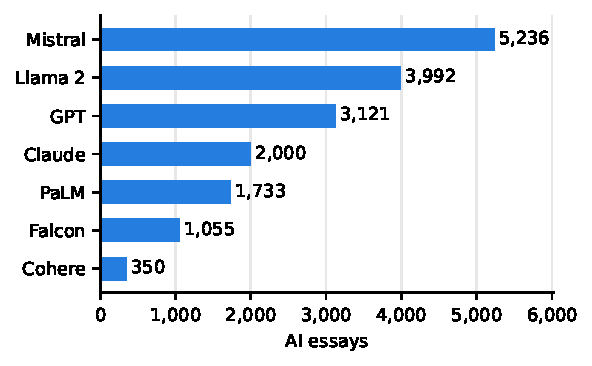
\includegraphics[height=4.2cm]{counts_per_generator.pdf}
  \end{columns}
\end{frame}

% =====================================================================
%  2 · Lengths
% =====================================================================
\kicker{Text length}
\begin{frame}{Text length: human vs.\ AI}
  \begin{columns}[T,onlytextwidth]
    \column{0.52\textwidth}
      \centering
      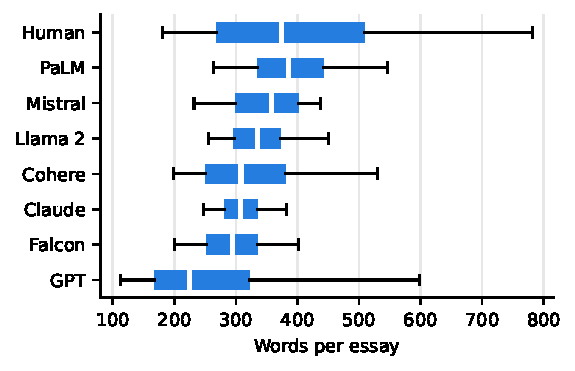
\includegraphics[height=4.6cm]{length_per_generator.pdf}
    \column{0.44\textwidth}
      \small
      \begin{itemize}
        \item Median words, human: 374
        \item Median words, AI: 328
        \item Shortest human essay: 143 words
        \item AI essays shorter than 143 words: 525
        \item ROC-AUC with length only: 0.72
        \item ROC-AUC with prompt only: 0.72
      \end{itemize}
  \end{columns}
\end{frame}

% =====================================================================
%  3 · Generators & splits   (Zahlen: src/splits.py, results/week1/)
% =====================================================================
\kicker{Splits}
\begin{frame}{Generators, random split and LOGO folds}
  \begin{columns}[T,onlytextwidth]
    \column{0.42\textwidth}
      \centering\small
      \renewcommand{\arraystretch}{1.15}
      \begin{tabular}{@{}lrr@{}}
        \toprule
        \textbf{Generator} & \textbf{Essays} & \textbf{In test} \\
        \midrule
        Mistral 7B        & 5{,}236 & 1{,}047 \\
        Llama 2 (7B, 70B) & 3{,}992 & 798 \\
        GPT (3.5, 4)      & 3{,}121 & 624 \\
        Claude            & 2{,}000 & 400 \\
        PaLM              & 1{,}733 & 347 \\
        Falcon 180B       & 1{,}055 & 211 \\
        \rowcolor{hkaStripe}
        Cohere            & 350     & \muted{train only} \\
        \midrule
        Human             & 26{,}058 & 5{,}212 \\
        \bottomrule
      \end{tabular}
    \column{0.54\textwidth}
      \small
      \begin{itemize}
        \item \textbf{Generator = model family:} variants merged, so a held-out model is truly unseen
        \item \textbf{Selection:} $\geq$\,1{,}000 essays $\Rightarrow$ \highlight{6 LOGO folds}; Cohere stays in training only
        \item \textbf{Random split:} 70/10/20 train/val/test, stratified by generator, seed 42
        \item \textbf{LOGO fold $G$:} train/val = random train/val without $G$; test = random test, human $+$ $G$ only
        \item \textbf{Paired comparison:} same test essays in both settings, only difference is whether $G$ was seen
      \end{itemize}
  \end{columns}
\end{frame}

% =====================================================================
%  4 · Metrics   (festgelegt in src/metrics.py)
% =====================================================================
\kicker{Metrics}
\begin{frame}{Evaluation metrics}{Fixed before the first model is trained}
  \begin{kvtable}
    \kv{Positive class}{AI-generated (\texttt{label} = 1)}
    \kvred{Main}{\textbf{ROC-AUC}: threshold-free, independent of the class ratio (varies per fold), Kaggle metric}
    \kv{Second}{\textbf{F1} (AI class): threshold = max.\ F1 on the validation split, never tuned on test}
    \kv{Additional}{\textbf{TPR @ 1\,\% FPR}: AI essays caught when $\leq$\,1\,\% of human essays are falsely flagged}
    \kv{Not used}{Accuracy: always predicting ``human'' already scores 96\,\% on the Falcon fold}
    \kv{Reported on}{Test part of the random split and of each LOGO fold; 95\,\% bootstrap CI for ROC-AUC}
  \end{kvtable}
\end{frame}

% =====================================================================
%  5 · Next steps & open questions
% =====================================================================
\kicker{Next week}
\begin{frame}{Next steps and open questions}
  \begin{columns}[T,onlytextwidth]
    \column{0.48\textwidth}
      \small
      \textbf{Next week}
      \begin{itemize}
        \item Baseline: TF-IDF (character n-grams) + logistic regression
        \item Evaluate on the random split and all 6 folds
        \item Set up GPU environment
      \end{itemize}
    \column{0.48\textwidth}
      \small
      \textbf{Open questions}
      \begin{itemize}
        \item Hold out by model family or by single model?
        \item How do we handle prompts that are mostly human or mostly AI?
      \end{itemize}
  \end{columns}
\end{frame}

\end{document}
